\documentclass[12pt,a4paper,abstract=on,parskip=full]{scrartcl}
\usepackage{a4wide}
\usepackage[T1]{fontenc}
\usepackage[french]{babel}
\usepackage[babel=true]{csquotes} % guillemets français
\usepackage{graphicx}
\graphicspath{{Images/}}
\usepackage{color}
\usepackage{hyperref}
\hypersetup{colorlinks,linkcolor=,urlcolor=blue}
\usepackage{fontspec}
\usepackage[svgnames]{xcolor}
\defaultfontfeatures{Ligatures=TeX}
\usepackage{amsmath}
\usepackage{amssymb}
\usepackage{minted}
\usepackage{enumitem}
\usepackage{amsthm}
\usepackage{url}
\newtheorem*{remark}{Remarque}
\usepackage[nottoc,notlot,notlof]{tocbibind}

%____USER COMMANDS___________
\newcommand{\HRule}[1]{\rule{\linewidth}{#1}}
%____________________________

\newfontfamily\subsubsectionfont[Color=black]{Fetamont}
\setkomafont{title}{\normalfont\subsubsectionfont}


\titlehead{\centering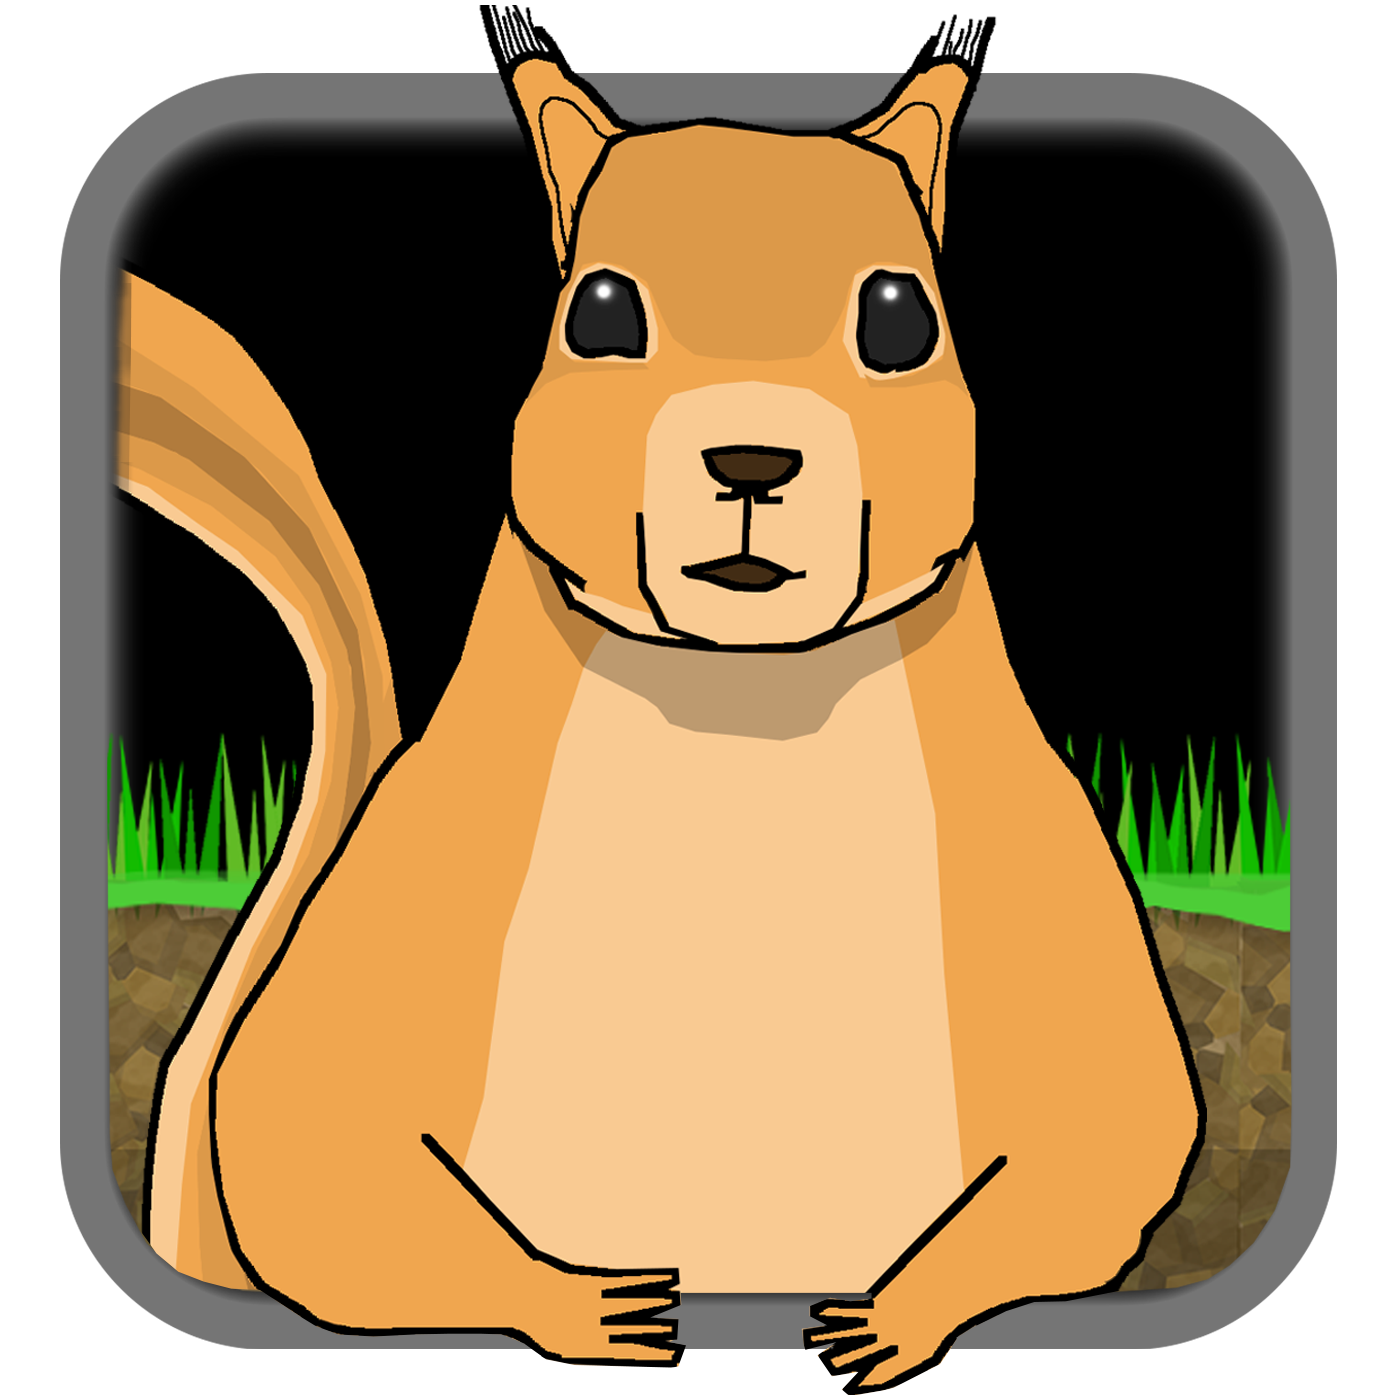
\includegraphics[width=4cm]{icon_squiro.png}}
\title{ \normalsize Développement Mobile
        \HRule{0.5pt} \\ [0.5cm]
        \LARGE \textbf{\uppercase{Rapport de projet : SQUIRO}}
        \HRule{0.5pt} \\ [0.5cm]
        \normalsize \today \vspace*{5\baselineskip}}
\author{Gonowree Bryan - M1 Informatique \\ [0.5cm]
		Université de La Réunion}
\date{\today}



\begin{document}

%____Première page____
\maketitle
\bigskip
%% Le résumé:
\begin{abstract}
Dans ce rapport, je tente d'expliquer la façon dont le projet "Squiro" a été conçu en soulevant les points les plus importants de la conception et en soulignant quelques subtilités. En complément et pour plus d'informations, je vous invite à vous réferer au code source de l'application, en particulier aux classes ".java" du dossier [src].
\end{abstract}

\thispagestyle{empty}
%___fin première page____

\clearpage

\tableofcontents
\setcounter{page}{1}
%Ajoute une section introduction qui ne sera pas numérotée mais affichée dans la table des matières
\section*{Introduction}
\addcontentsline{toc}{section}{Introduction}

"Squiro" est un dérivé du mot anglais "squirrel" qui signifie "écureuil" en français. C'est le nom du personnage principal du jeu, il constitue le point de départ du projet.
En effet, l'idée de base était de créer un jeu utilisant le capteur accéléromètre pour la plateforme mobile Android, dans lequel, un petit personnage, en l'occurence Squiro, avancerait sur des plateformes en essayant d'éviter des "obstacles". Un score étant incrémenté à chaque obstacle évité.

Finalement, après extrapolation, l'idée d'obstacles a été implémentée comme étant des "trous" dans lequel Squiro est censé tomber pour continuer à avancer. Les plateformes, quant à elles sont tout simplement constitués
de terre et d'herbe, comme le serait le milieu naturel d'un petit écureuil courant dans l'herbe. 

Après avoir posé les idées de base du projet,
la phase de conception technique et l'implémentation des fonctionnalités débutent.
Ce sont sur ces dernières que nous allons nous focaliser dans ce rapport.


\section{Architecture générale de l'application}
\subsection{Dossiers et classes}
\label{section:hello} % pour faire référence à la section ailleurs (\ref{...} voir plus bas)

L'application a été décomposée en de multiples dossiers et classes afin d'améliorer la lisibilité du programme mais aussi pour des raisons de maintenance et d'ajout de fonctionnalités futures.
Elle a, donc, été structurée comme ceci :

%Liste des classes et des dossiers
\begin{itemize}[label=$\bullet$, nosep]
\item\ \textit{\color{blue} MainActivity.java}

\item\ \textbf{[GameEngine]}
\begin{itemize}[nosep]
\item\ \textit{\color{blue} GameView.java}
\end{itemize}

\item\ \textbf{[GameOver]}
\begin{itemize}[nosep]
\item\ \textit{\color{blue} GameOverActivity.java}
\end{itemize}

\item\ \textbf{[Graphics]}
\begin{itemize}[nosep]
\item\ \textit{\color{blue} Obstacle.java}
\item\ \textit{\color{blue} Squiro.java}
\end{itemize}

\item\ \textbf{[Maps]}
\begin{itemize}[nosep]
\item\ \textit{\color{blue} MapsActivity.java}
\end{itemize}

\item\ \textbf{[ScoreList]}
\begin{itemize}[nosep]
\item\ \textit{\color{blue} MyArrayAdapter.java}
\item\ \textit{\color{blue} Score.java}
\item\ \textit{\color{blue} ScoresListActivity.java}
\end{itemize}

\item\ \textbf{[Sounds]}
\begin{itemize}[nosep]
\item\ \textit{\color{blue} SoundManager.java}
\end{itemize}

\end{itemize}


\hspace{50pt} \textbf{[ * ]} : Dossier \hspace{50pt} {\color{blue} \textit{*.java}} : Classe Java




\subsection{Rôles des classes}
Comme énoncé dans le résumé, les descriptions suivantes ne sont pas totalement exhaustives. Elles se complètent donc avec une lecture du code associé à ces classes.  
\subsubsection[MainActivity]{\color{blue} MainActivity}
C'est l'activité qui est chargé initialement lors du lancement de l'application. Elle a pour but de commencer l'écoute des évènements liés à l'accéléromètre de l'appareil, de lancer le jeu au départ et de gérer certaines situations spécifiques au jeu.
Ces situtations sont par exemple, le relancement du jeu ou la sortie de l'application.
De plus, depuis elle on peut accéder à la liste des scores par le biais de la barre de menu en haut du jeu.

\begin{remark}[Launch Mode]
Cette activité est en mode "singleInstance", cela évite à l'appareil de constamment recréer de nouvelles instances du jeu. En particulier cela évite le rechargement des bitmaps et donc contribue à la fluidité de l'application. 
\end{remark}

\subsubsection[GameView]{\color{blue} GameView}
Cette classe gère tout le traitement lié au jeu en lui-même en chargeant les bitmaps, générant les obstacles et déplaçant le personnage.
C'est la classe la plus conséquente de l'application.
Elle exécute donc ses instructions dans un thread séparé en implémentant la classe Runnable. 

\subsubsection[GameOverActivity]{\color{blue} GameOverActivity}
Cette activité représente la vue "Game Over" lorsque l'on perd au jeu. En plus de cela, elle est aussi chargée de récupérer le score, la position, le pseudo du joueur et de les enregistrer.

\begin{remark}[Recents Panel]
Cette activité étant transparente, si on y accède depuis le panneaux des applications récentes, ses élements ne seront plus cohérents avec le background. Le "Look and Feel" de l'application étant donc atteint, les attributs noHistory et excludeFromRecents ont été mis à "true" dans les options de l'activité pour éviter cela.
\end{remark}

\subsubsection[Obstacle]{\color{blue} Obstacle}
Cette classe est la représentation d'une plateforme contenant un "trou" situé aléatoirement. Elle dispose d'une méthode draw qui permet de dessiner son obstacle dans un canvas.

\subsubsection[Squiro]{\color{blue} Squiro}
Cette classe est la représentation du personnage de Squiro. Elle est chargée de créer le personnage et de l'animer en fonction du mode choisi (en course ou sur place). Elle dispose d'une méthode draw qui permet de dessiner, dans un canvas, chaque frame du spritesheet choisi, chaque fois que celle-ci est appelée.

\subsubsection[MapsActivity]{\color{blue} MapsActivity}
Cette activité est appelée à chaque fois que l'utilisateur clique sur un score dans la liste des scores et que ce score dispose de données de location. Grâce à ces données, elle lance une Map des Google Play Services
situé sur la position obtenue, sur laquelle on peut voir le score, le pseudo et la position du joueur associé à l'élement de la liste selectionné.

\subsubsection[MyArrayAdapter, Score et ScoresListActivity]{{\color{blue} MyArrayAdapter}, {\color{blue} Score} et {\color{blue} ScoresListActivity}}
MyArrayAdapter est l'adapteur qui gèrera tous les scores associé à la listView de l'activité ScoresListActivity.
La classe Score étant la représentation d'un score contenant des attributs sur le détenteur du score, comme le pseudo et sa position géographique.
ScoresListActivity, quant à elle, a pour but de charger les scores dans la base de données (SharedPreferences), de les afficher dans une listView et de rediriger l'utilisateur vers MapsActivity lors d'un clic sur un élement.

\subsubsection[SoundManager]{\color{blue} SoundManager}
Cette classe gère les sons liés au jeu, comme les sons d'ambiances, de chute dans un "trou" ou encore de perte.
Elle veile à ce que les sons ne soit pas en conflits les un avec les autres et propose des méthodes pour les jouer à tout moment.

\section{Détails techniques du code}

Dans cette section, sont présentés des implémentations en Java de certaines parties de l'application. Elles ont été séléctionnées pour leur caractère que j'ai considéré comme étant complexe, délicat ou encore non-commun.

\subsection{GameView, une SurfaceView Runnable}

Pour la vue de notre jeu, SurfaceView s'est imposée comme étant la meilleure solution pour réaliser un jeu simple et accueilir quelques éléments graphiques. En effet, SurfaceView permet de déléguer toute la partie dessin à un thread autre que celui de l'UI-Thread principal.

Pour réaliser cette fonctionnalité, la technique choisie a été de rendre cette SurfaceView, elle-même, Runnable, puis de l'associer à un nouveau Thread et enfin de réaliser tout le code graphique dans la méthode run() comme explicité ci-dessous.

\begin{minted}{java}
import ...;
public class GameView extends SurfaceView implements Runnable {
   [...]
   SurfaceHolder holder;
   private boolean playing;	
   public GameView(Context context) {
      super(context);
      this.context = context;
      holder = getHolder();
      playing = true;
      Thread renderThread = new Thread(this);
      renderThread.start();     
      [...]
   }    
   @Override
   public void run() { 
      while(playing) {
         if(!holder.getSurface().isValid()) {
            continue;
         }
         //-- Définition d'un canvas, et verrouillage le temps 
         //que l'on dessine dessus
         Canvas canvas = holder.lockCanvas();                        
         //--------------------------------
         //* Execution du code de dessin *                                 
         //--------------------------------
         //-- Libération du dessin
         holder.unlockCanvasAndPost(canvas);           
      }
   }
}
\end{minted}

\subsection{Sauvegarde de scores dans les SharedPreferences grâce à JSON}

Pour la sauvegarde des scores et des informations associées, la solution des SharedPreferences m'a semblé la plus sûre et la plus adaptée à la situation.
Cependant, le stockage de plusieurs valeurs dans les SharedPreferences peut sembler difficile de permier abord mais est en réalité très commode grâce à l'utilisation des JSONArray dont voici un exemple.

\begin{minted}{java}
SharedPreferences prefs = getApplicationContext().
getSharedPreferences(MainActivity.sharedPreferencesName, MODE_PRIVATE);

SharedPreferences.Editor editor = prefs.edit();

JSONArray scores = new JSONArray();

//Nous pouvons par exemple maintenant ajouter 
//des JSONArray à notre JSONArray scores afin de grouper 
//plusieurs informations dans un seul élement...
JSONArray actualPlayerInfos;
//--------------------------------------
//*  remplissage de actualPlayerInfos  *//
//--------------------------------------
scores.put(actualPlayerInfos);
//Conversion JSONArray -> String et push.
editor.putString("scores", scores.toString());
editor.commit();
//La récupération se fait très simplement
//grâce à la conversion String -> JSONArray
JSONArray newScores = new JSONArray(prefs.getString("scores", "[]"))
\end{minted}

\subsection{Nombre optimal d'obstacles à afficher sur l'écran}

Etant donné la faible limite moyenne du tas JAVA ("heap size") disponible pour les applications Android, il était nécéssaire de trouver un moyen de ne pas gaspiller la moindre mémoire allouée et ainsi d'éviter les "OutOfMemoryError".
En particulier, la situation devient encore plus critique lors de l'utilisation de bitmaps avec lesquels ce genre d'erreurs peut survenir très rapidement.
Dans notre situation, un mécanisme de synchronisation entre ajout et supression
d'obstacles à été mis en place. (Voir un peu plus bas.)

\begin{minted}{java}
int count = 0;
int periodicCount = count;
boolean obstaclesSynchronization = true;

//Execution du jeu
while(playing) {
   //Etape 1: Remplissage de l'écran. 
   if (obstaclesSynchronization) {
      count++;
      //On ajoute périodiquement des obstacles afin de remplir
      //l'écran, la périodicité est calculée de sorte que l'utilisateur
      //ait l'impression qu'il y ait une infinité d'obstacles qui défilent
      //petit à petit.
      if (count >= (periodicCount + (int) (obstacleHeight / defilSpeed))) {
         periodicCount = count;
         addNewObstacle();
      }
   }      
   //Etape 2: Passage en mode synchronisé.
   //A partir de maintenant dès qu'un obstacle sort vers le haut
   //on en ajoute un vers le bas.
   if (HigherObstacle.getY()<0) {
      if (obstaclesSynchronization)
         obstaclesSynchronization = false; //fin de l'étape 1.
      remove(HigherObstacle);
      addNewObstacle();
   }
   //De cette façon le nombre optimal d'obstacles sur l'écran est trouvé 
   //automatiquement en fonction de la taille de l'écran, ce nombre se veut
   //constant et la quantité de mémoire utilisée est par conséquent optimale.
}
\end{minted}

\subsection{Autres}

D'autres détails techniques sont tout aussi importants pour la bonne compréhension de ce projet. Cependant, ils ne seront pas explicités ici mais documentés dans le code source.
Nous avons par exemple, le mécanisme de \textbf{restart du jeu} qui ne recrée pas d'activités à chaque execution, l'\textbf{animation du personnage Squiro} grâce aux spritesheet ou encore l'implémentation de bornes pour donner l'\textbf{illusion d'une gravité dans le jeu}...

\section{Screenshots}

\vspace{12pt}
\hspace{5pt}
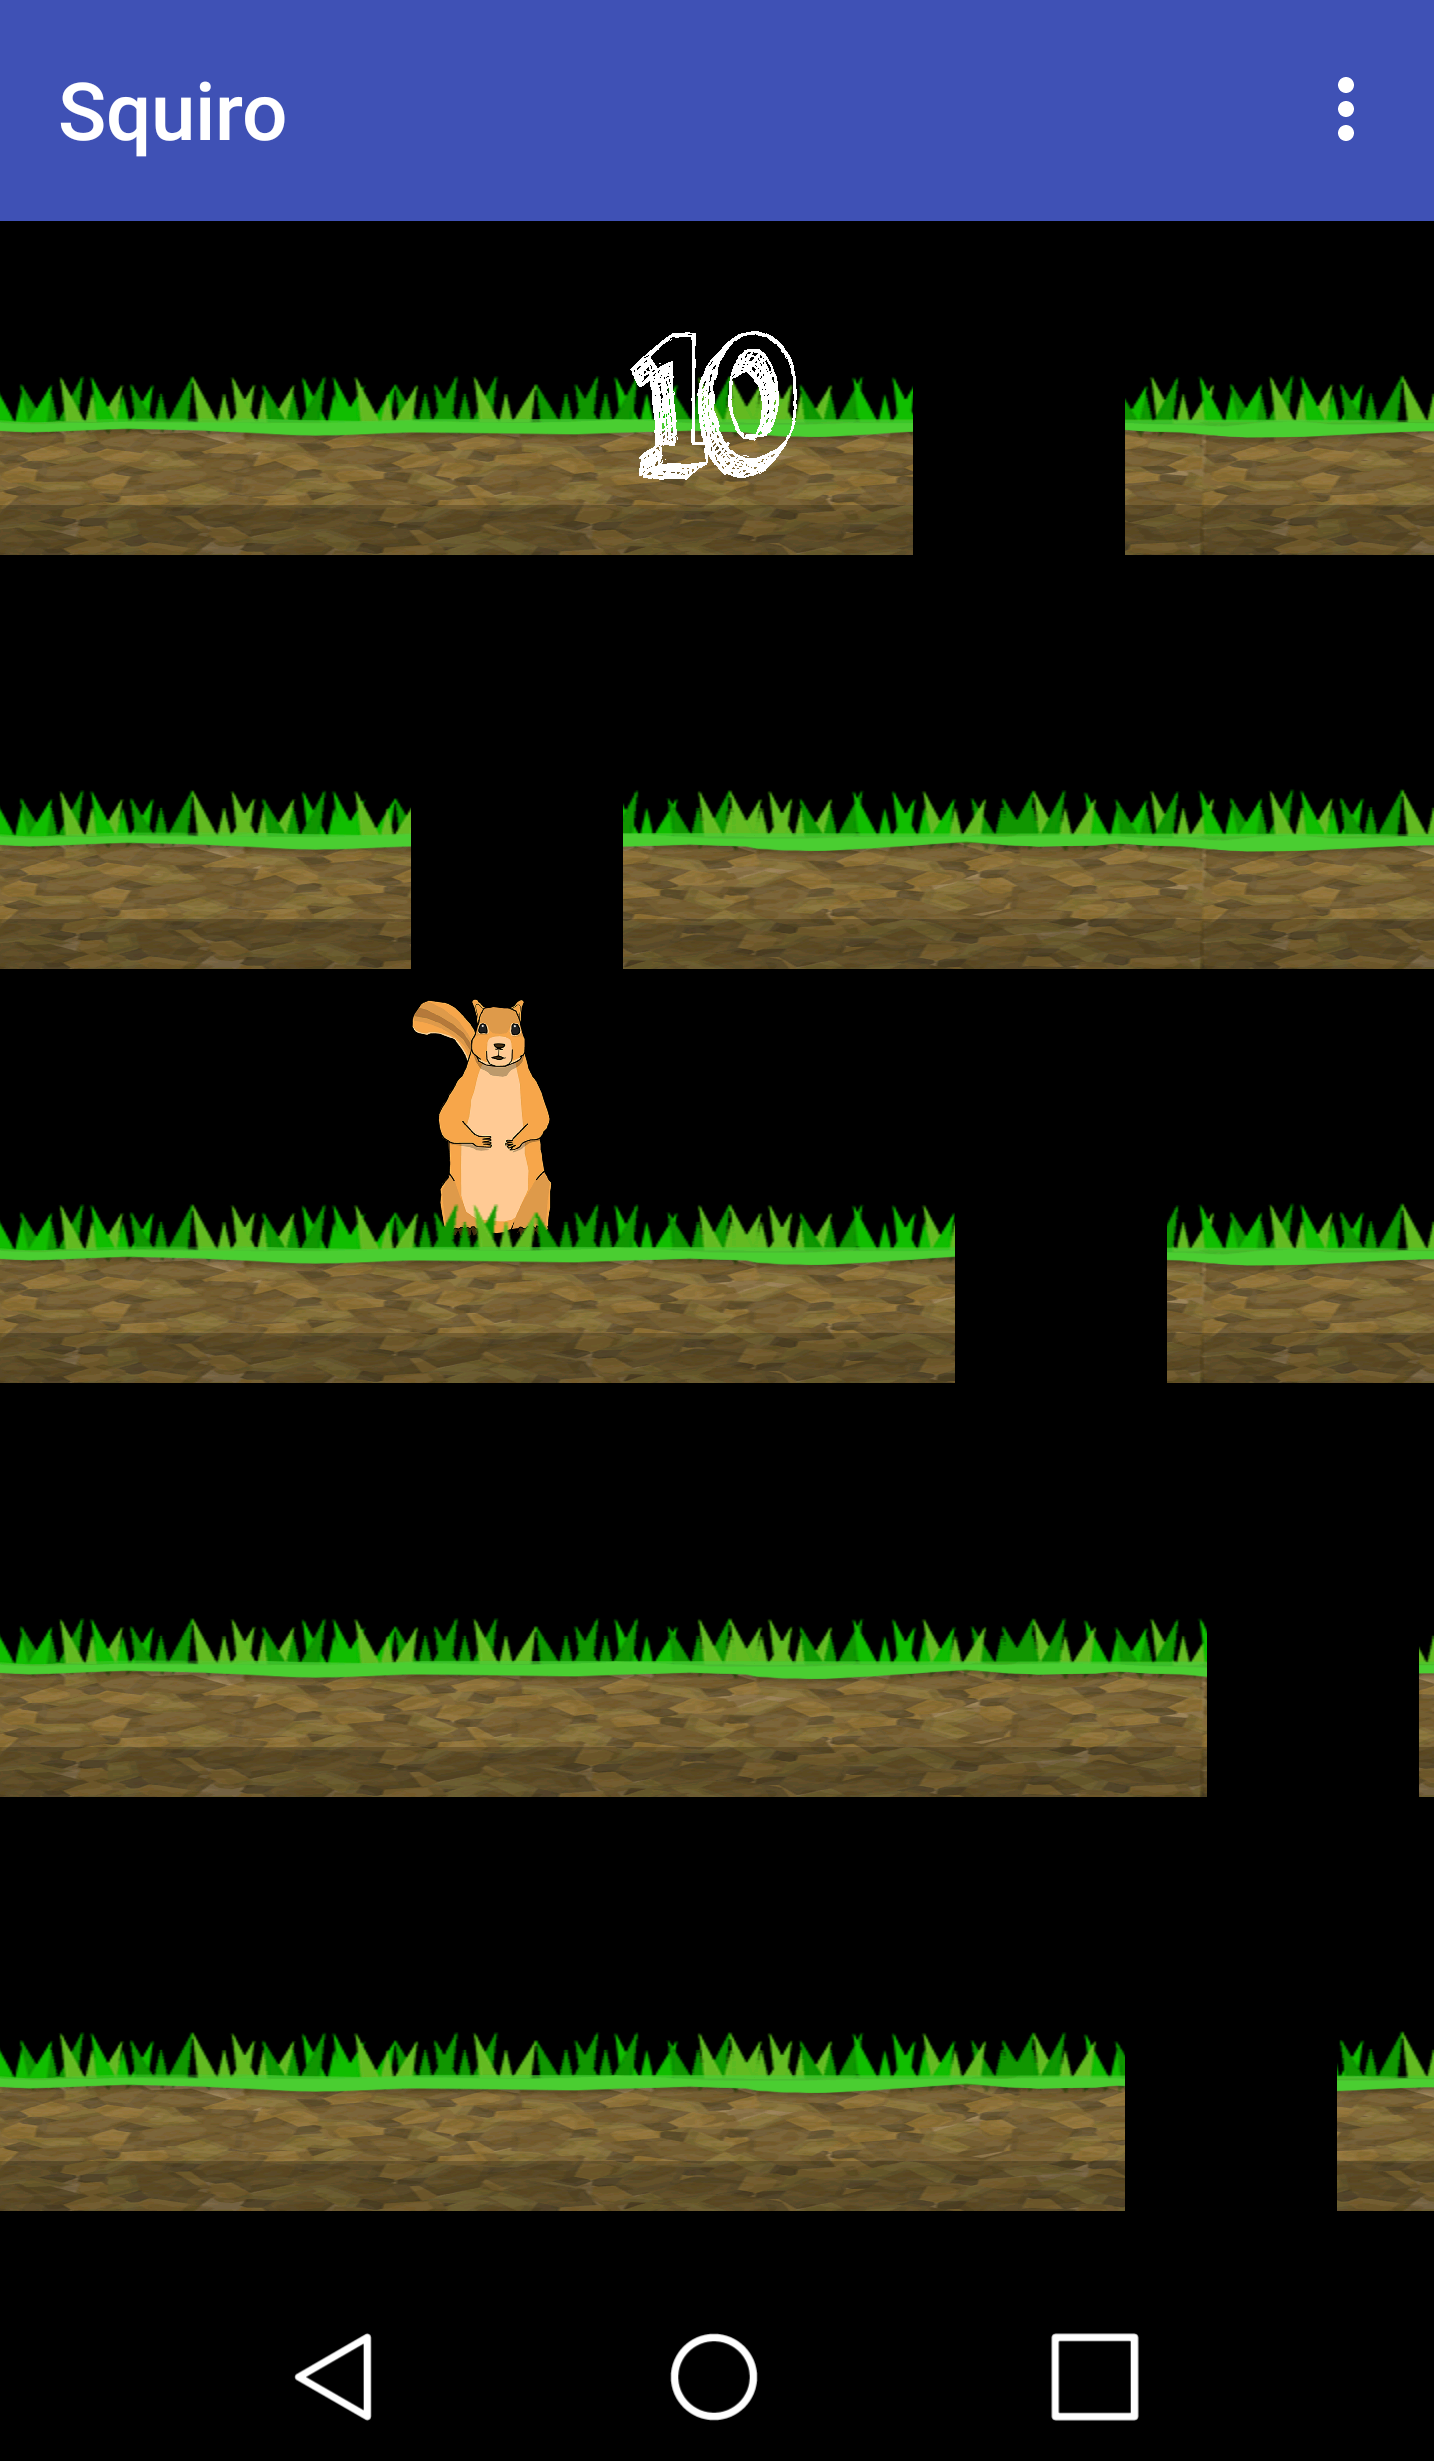
\includegraphics[width=5cm]{screenshot1.png}
\hspace{5pt}
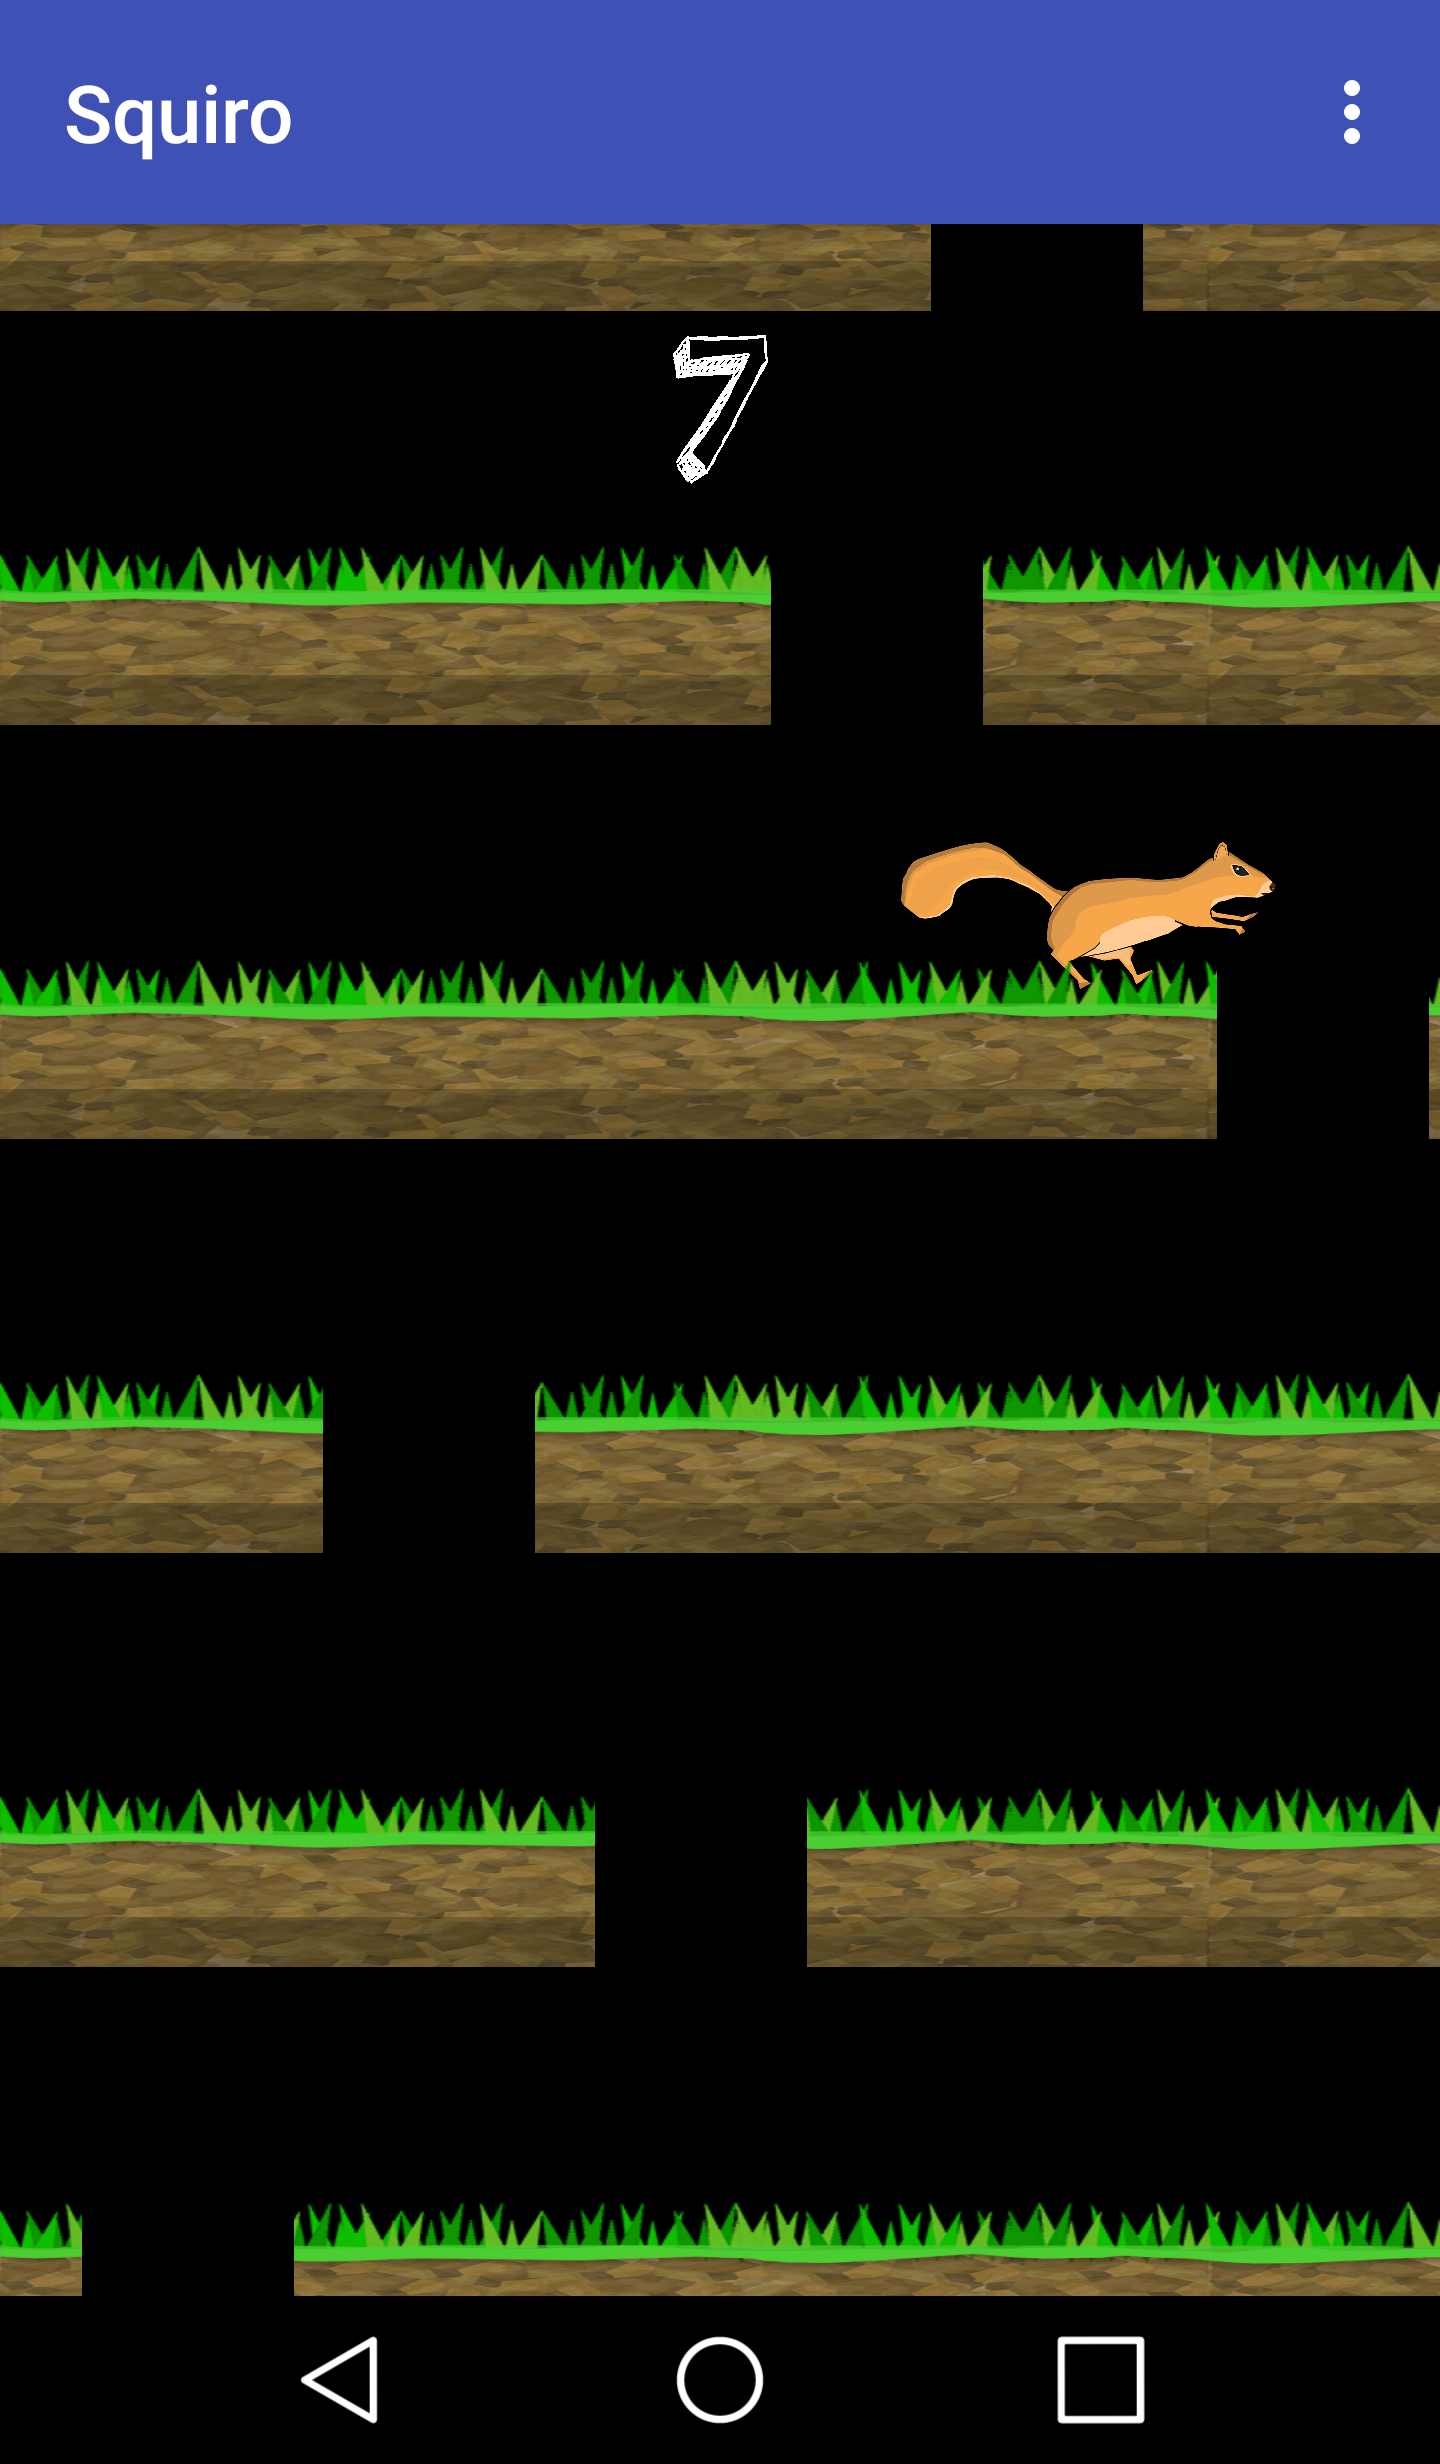
\includegraphics[width=5cm]{screenshot2.png}
\hspace{5pt}
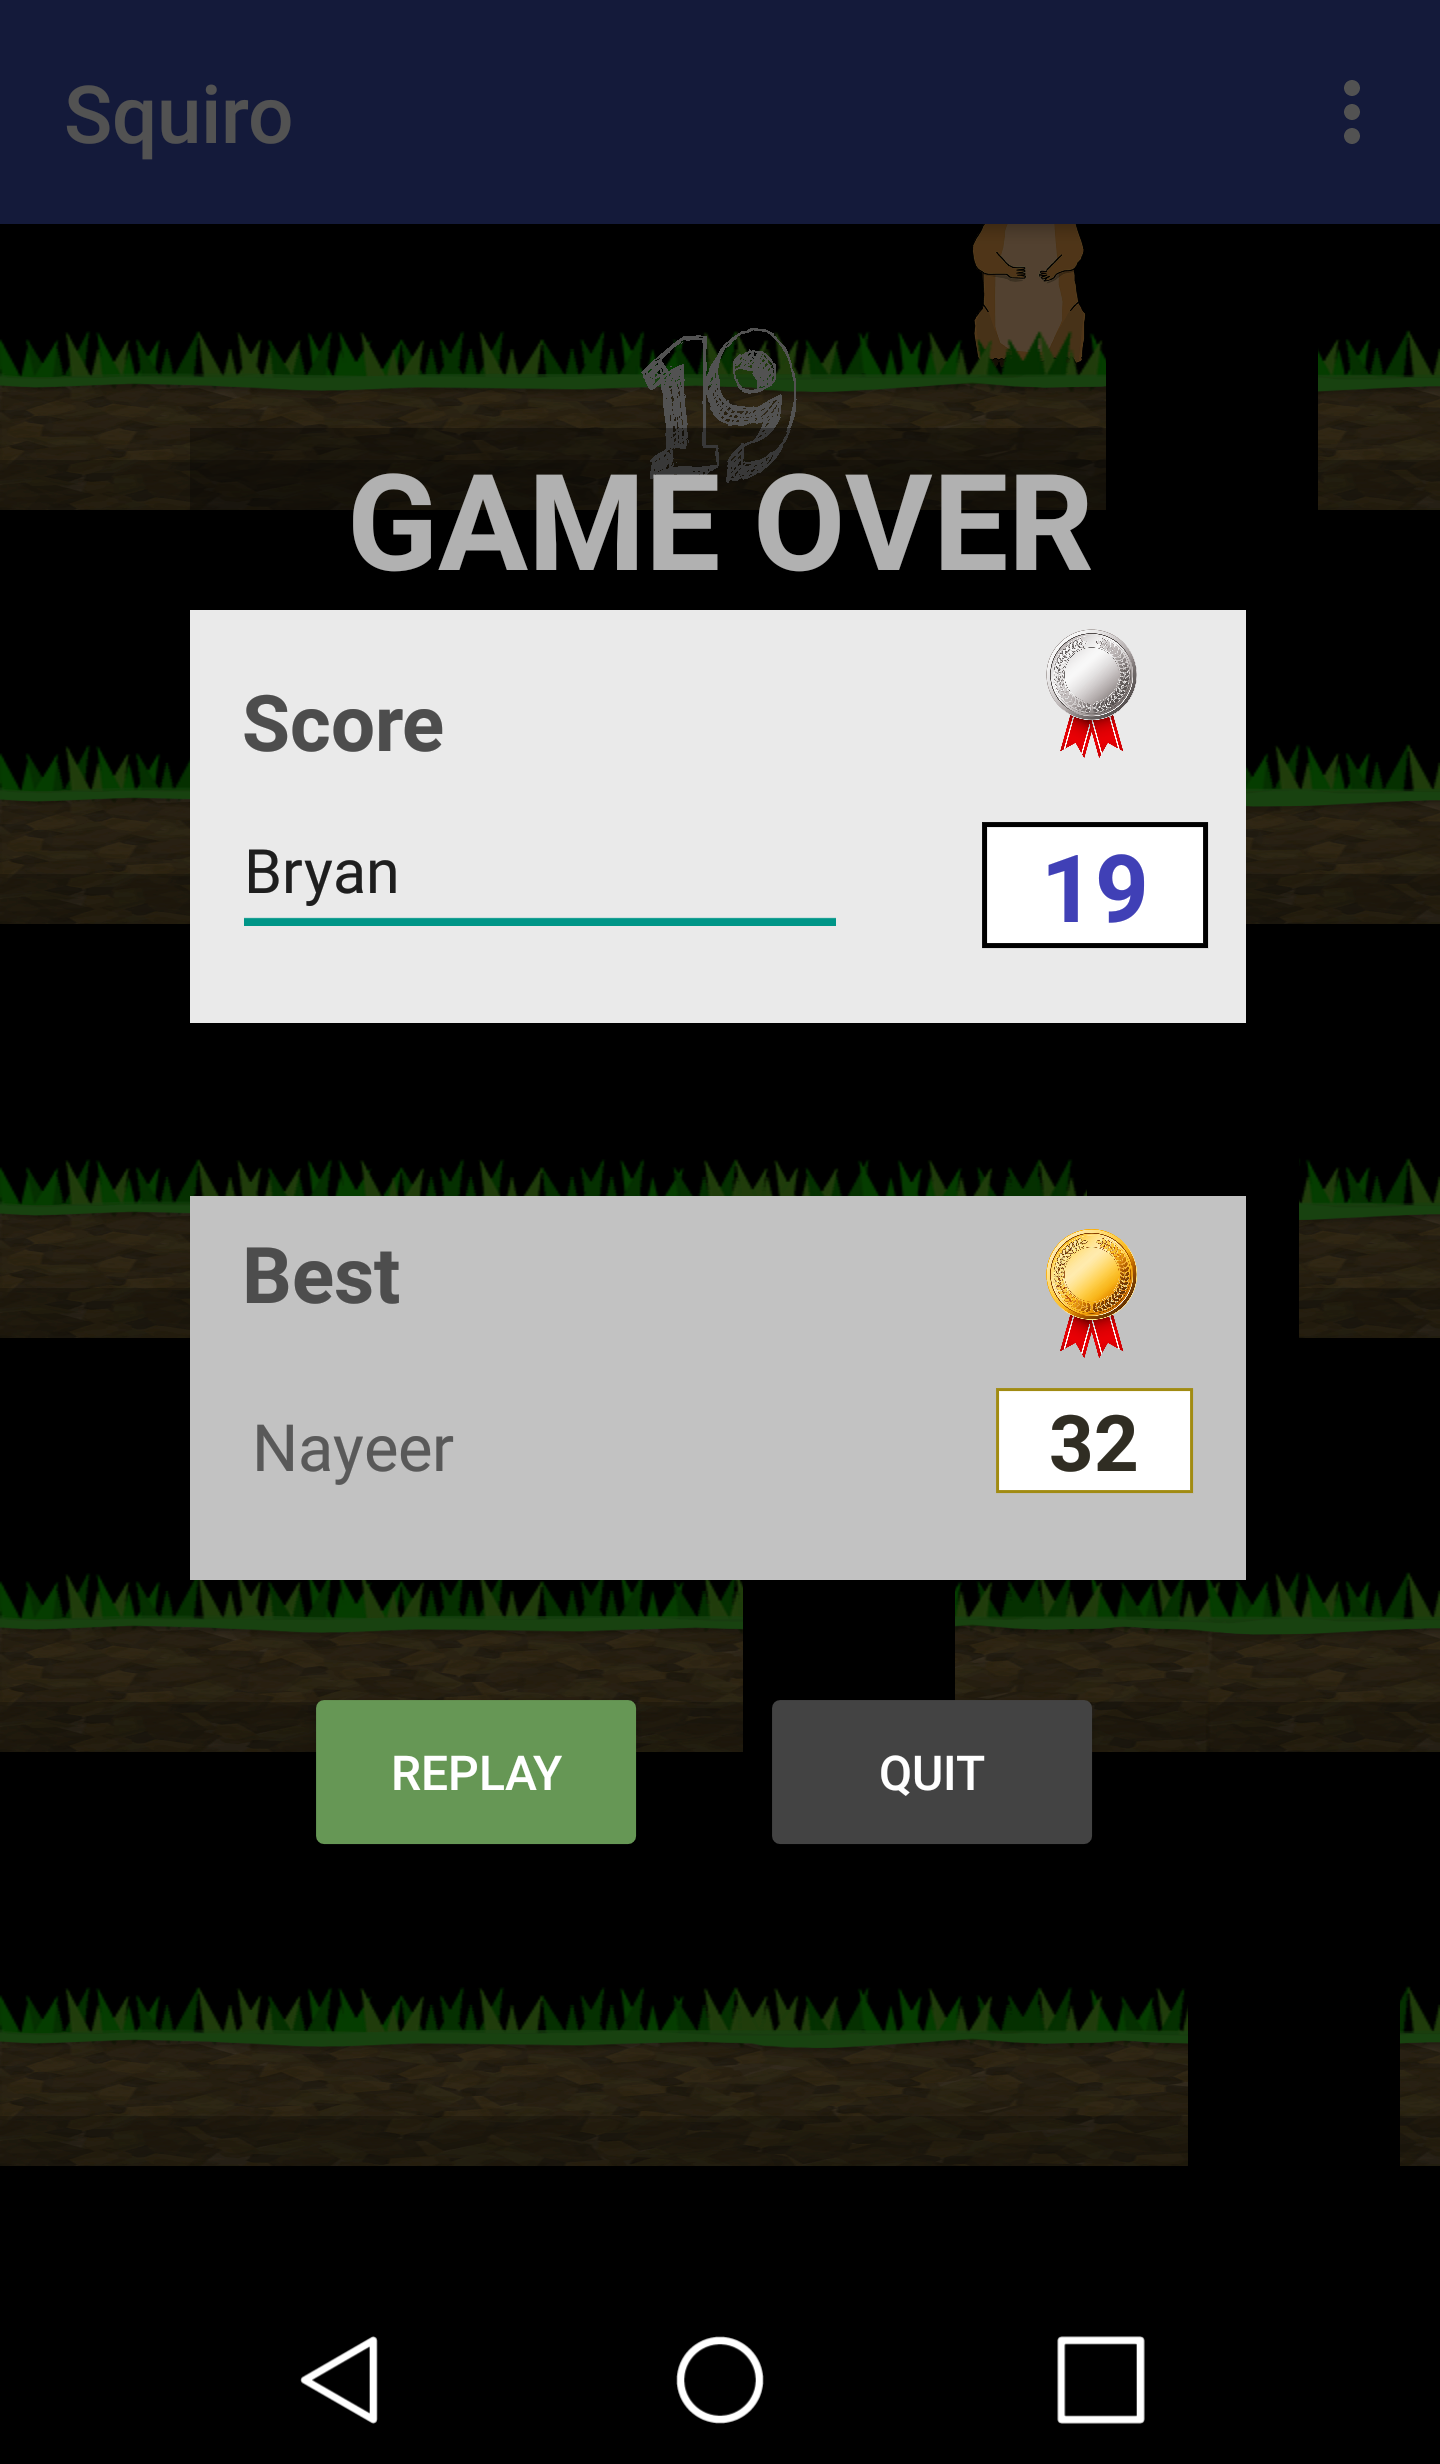
\includegraphics[width=5cm]{screenshot3.png}
\hspace{5pt}
\linebreak
\vspace{30pt}
\hspace{5pt}
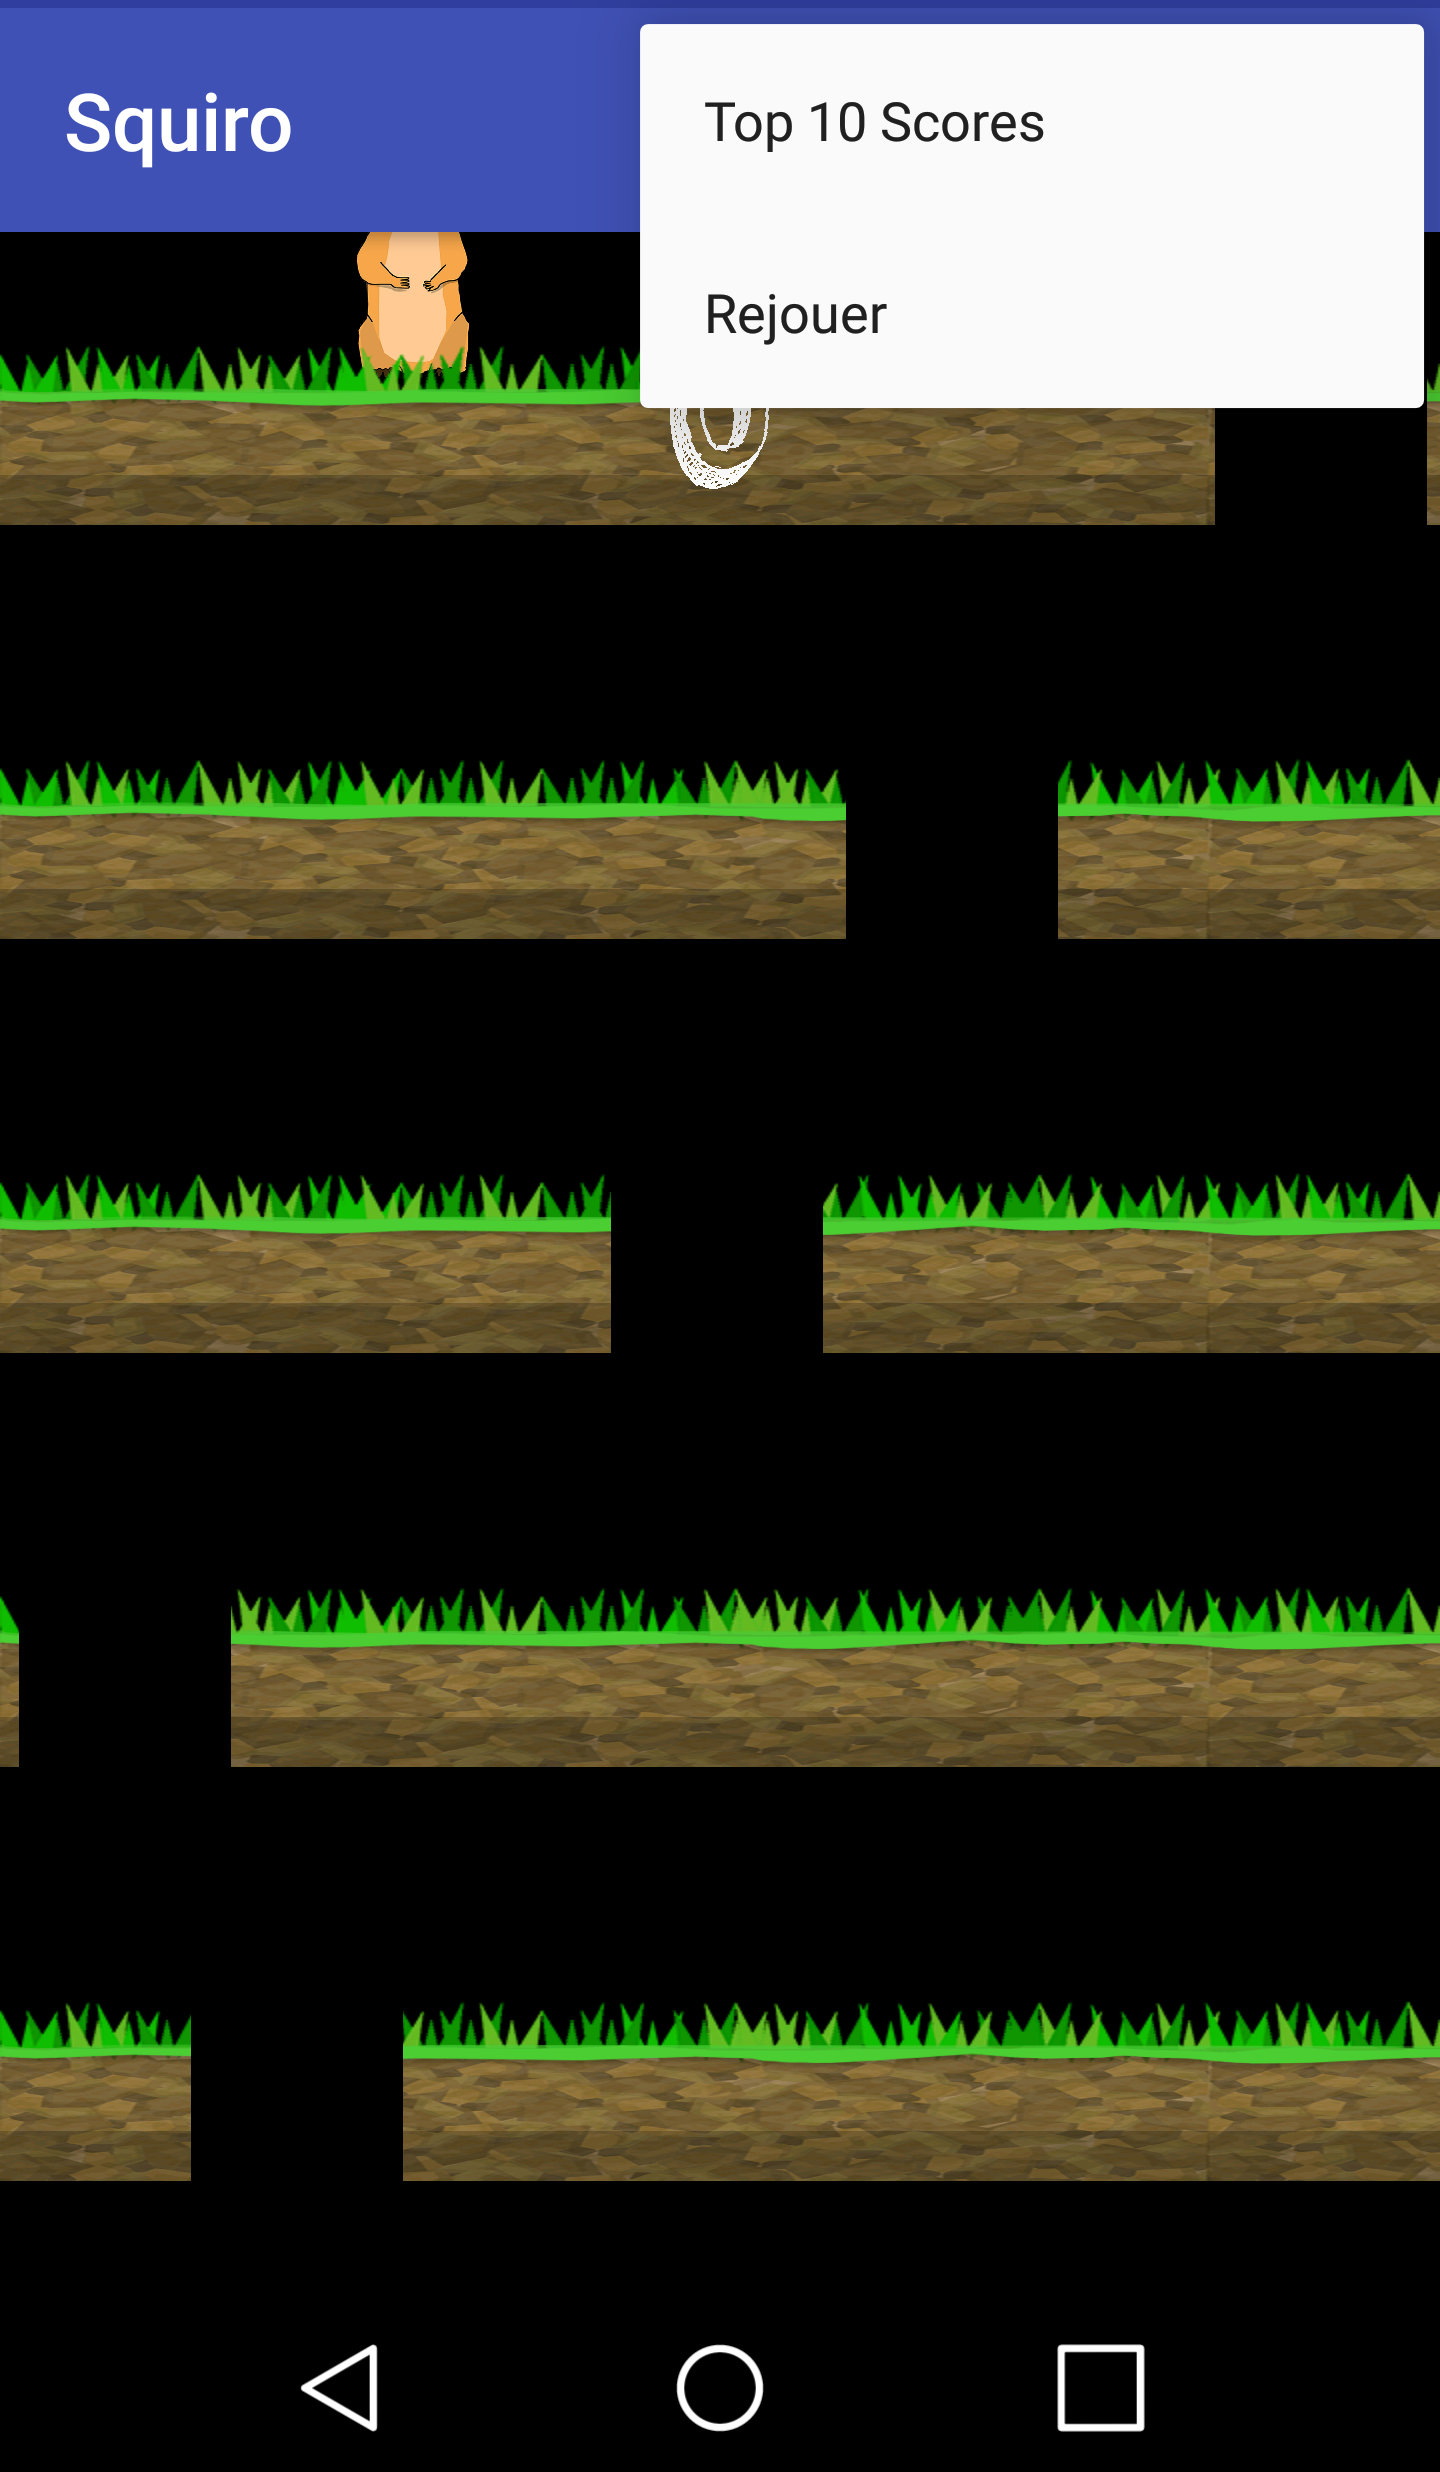
\includegraphics[width=5cm]{screenshot4.png}
\hspace{8pt}
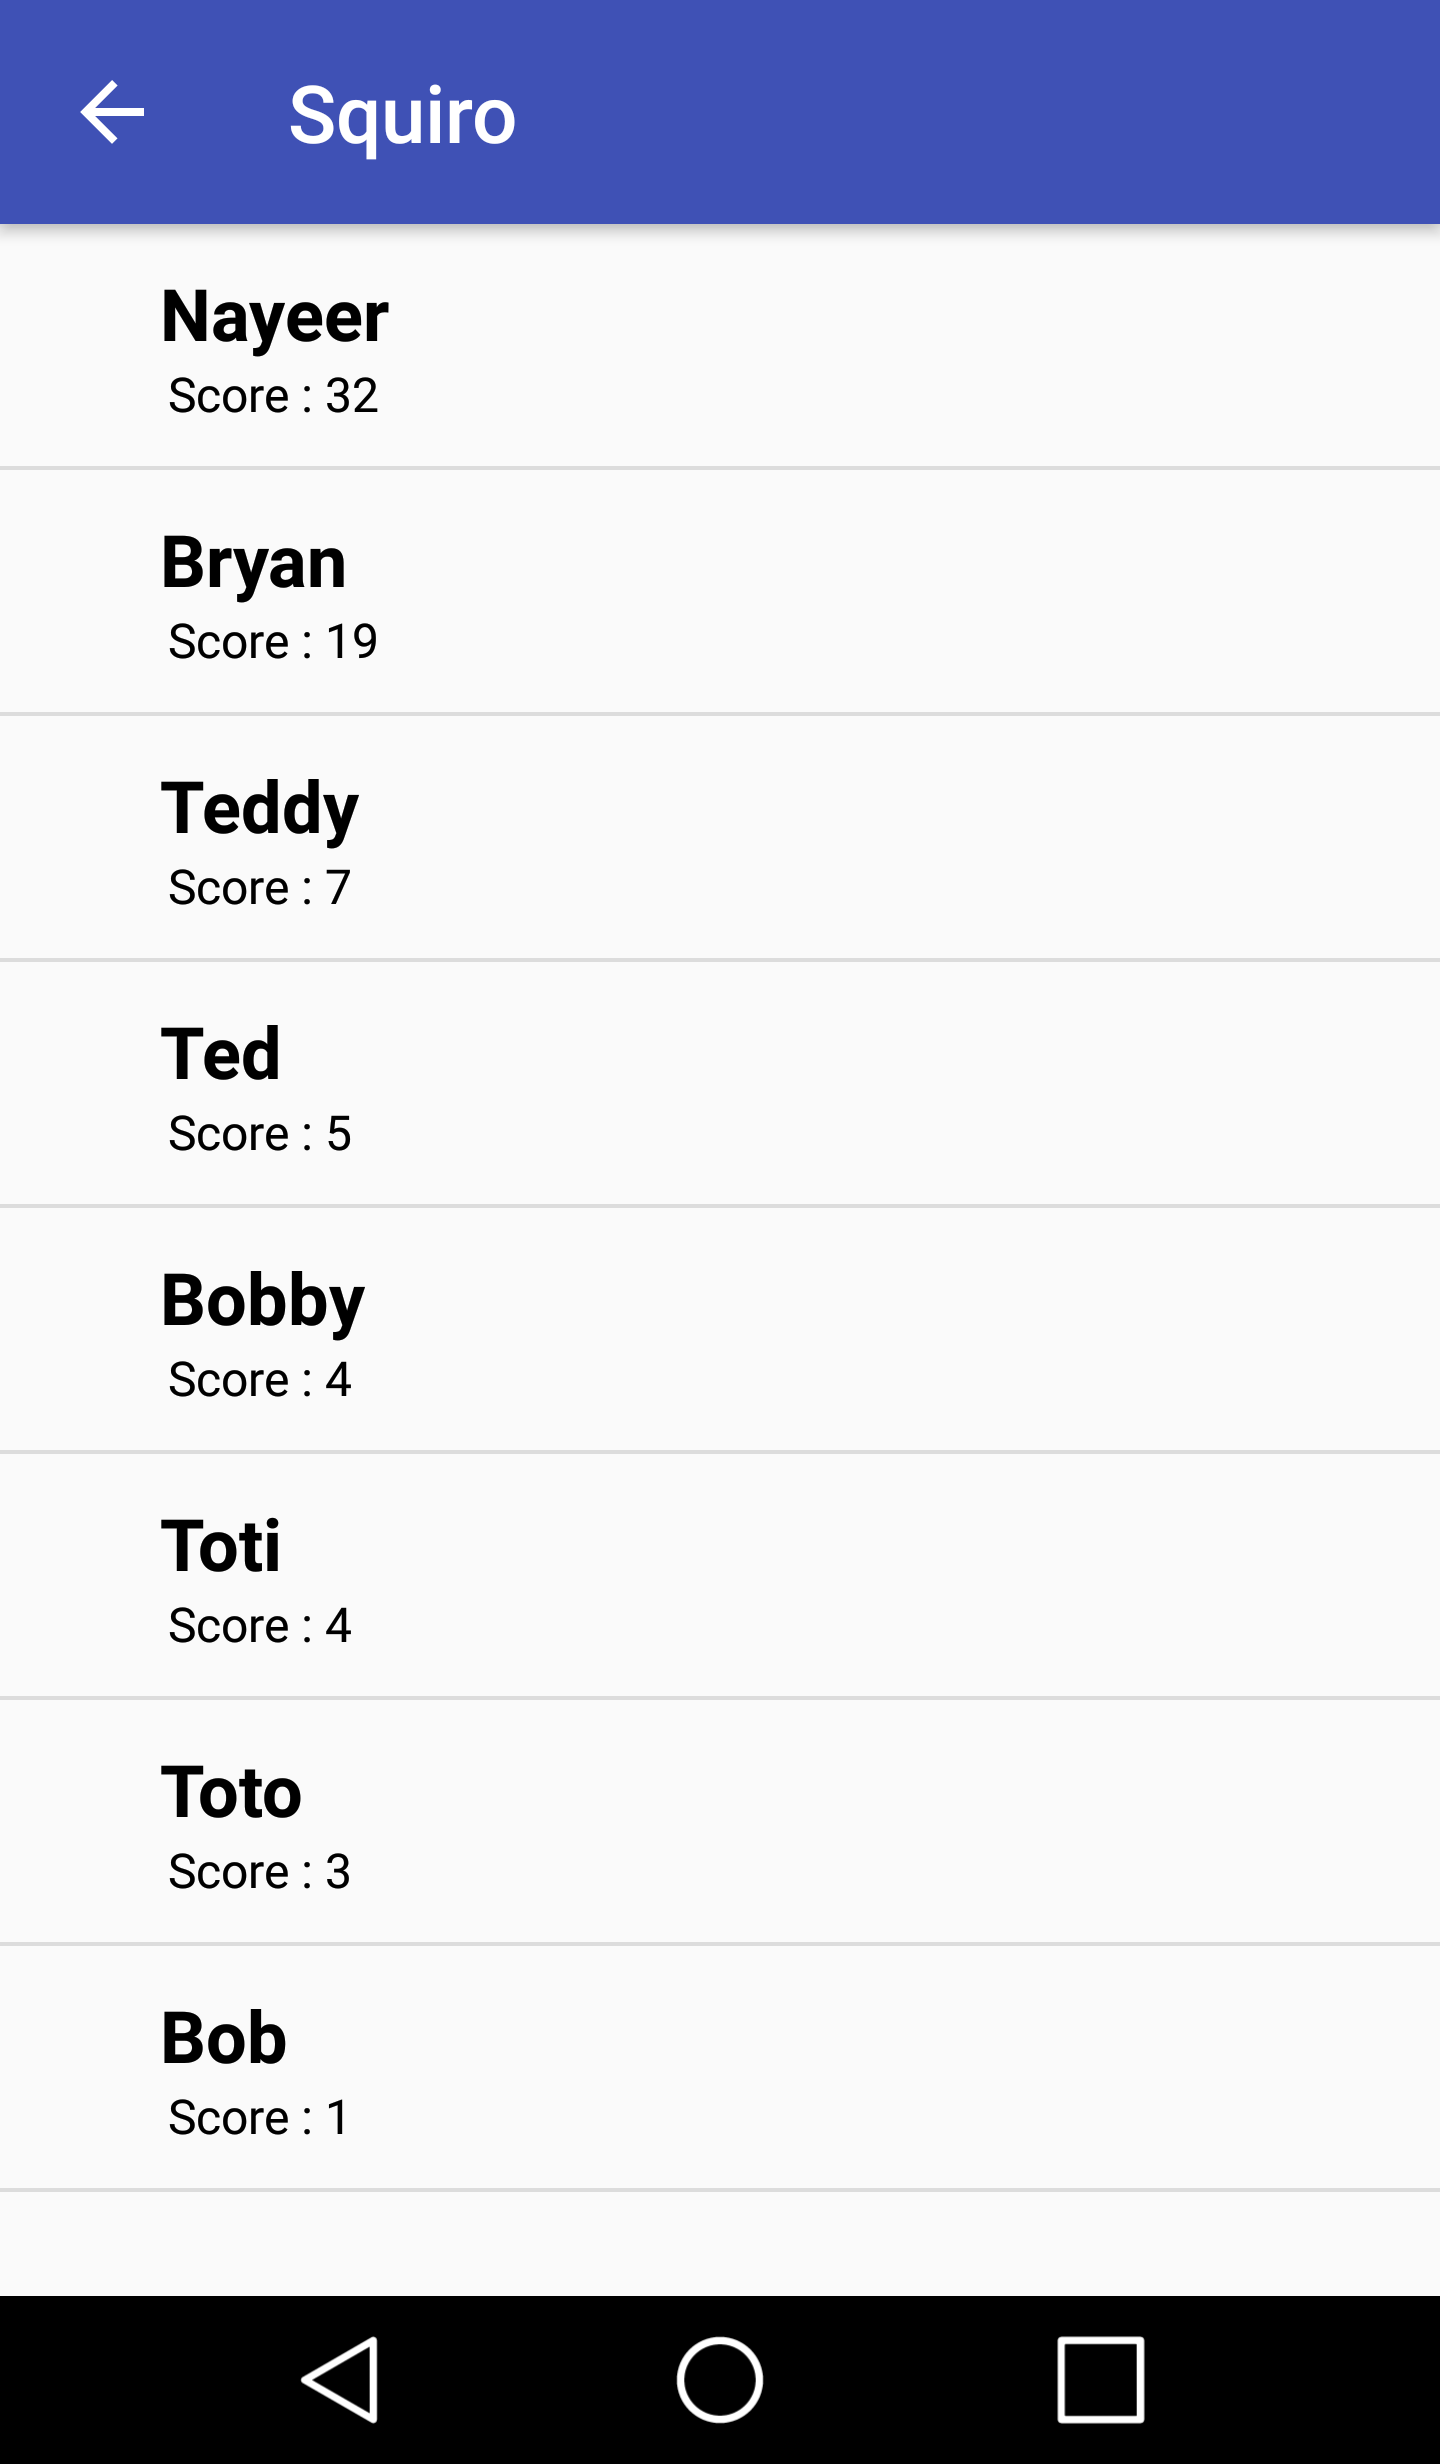
\includegraphics[width=5cm]{screenshot5.png}
\hspace{8pt}
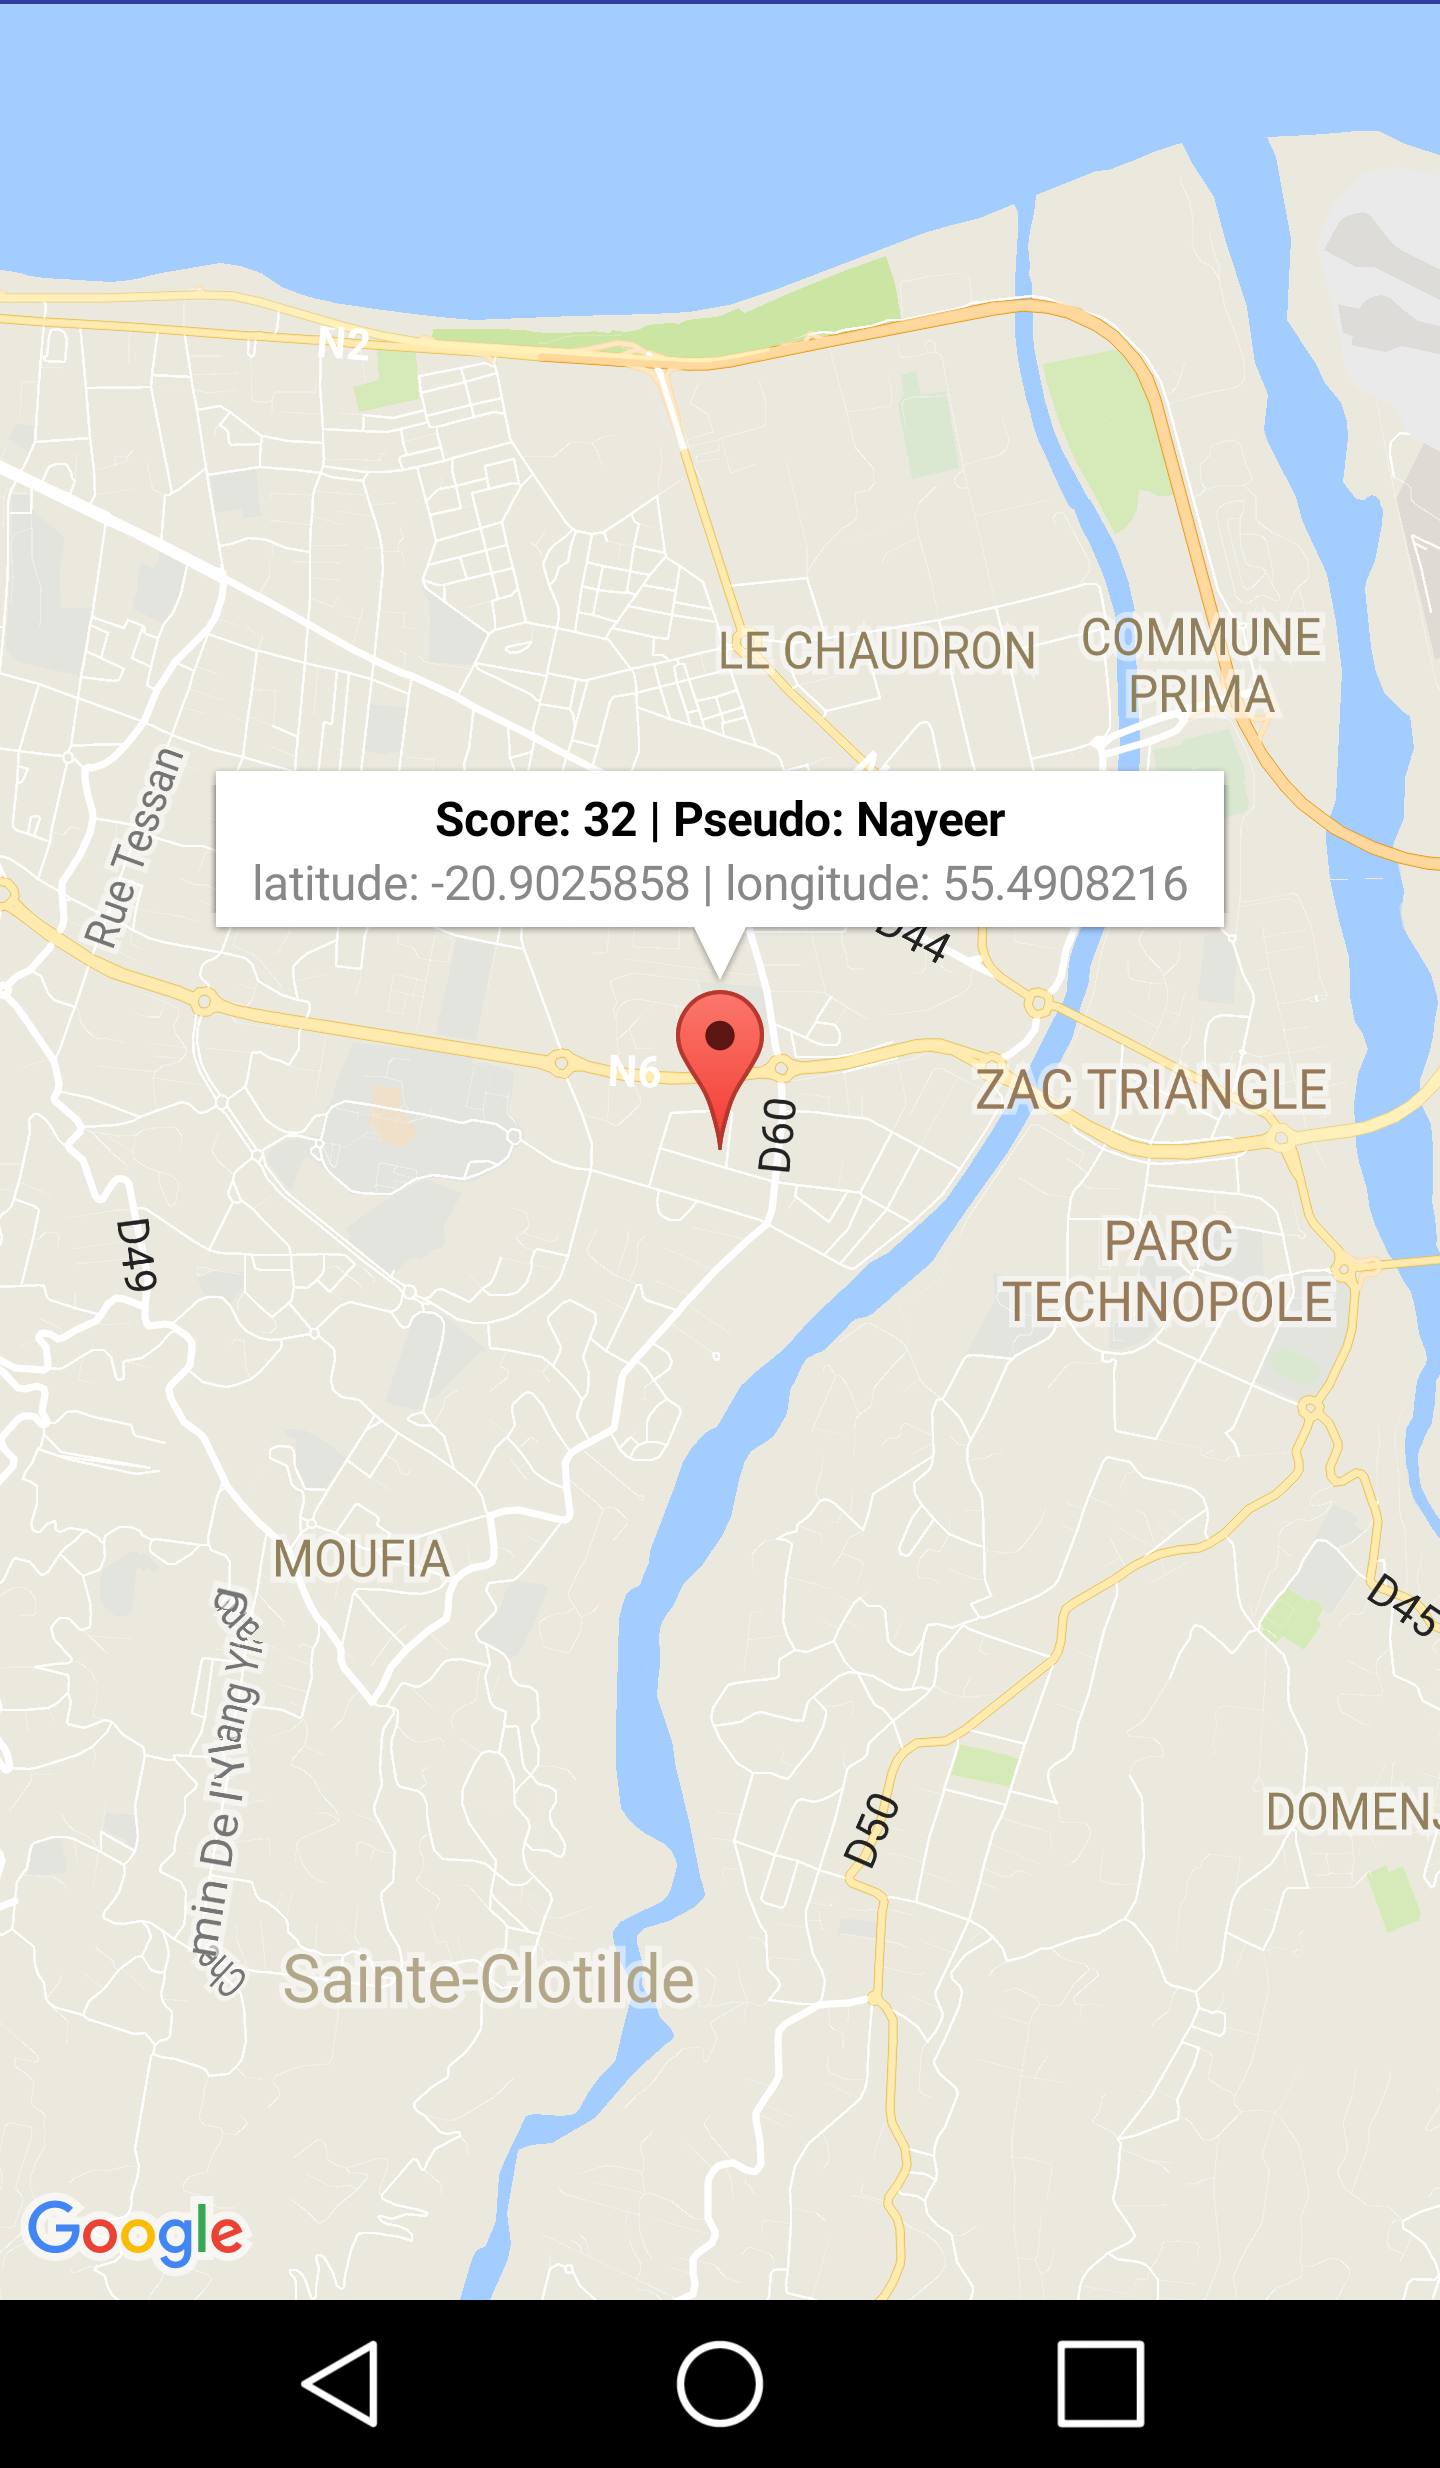
\includegraphics[width=5cm]{screenshot6.png}

\begin{remark}[Dessin]
Tous les bitmaps ont été dessinés "à la main" grâce à des logiciels de dessin assisté par ordinateur.
\end{remark}



%%% La bibliographie:
\nocite{*}
\bibliographystyle{plainurl}
\bibliography{ma_biblio}



\end{document}
